\section{Calibration details}
\label{app:calibration}

Table~\ref{tab:calibration} gives the full false-positive grid behind
Figure~\ref{fig:calibration}. We report two $\alpha$ regimes deliberately. The
\emph{family-wise} regime additionally divides $\alpha$ by the number of items,
holding a 0.05 rate across a whole screen. It controls family-wise error
across the screen but becomes more stringent per item as the screen grows,
reducing sensitivity at a fixed per-item sampling budget. Consequently, fewer
detected violations need not imply greater compatibility. The
\emph{per-item} regime holds per-item stringency constant in screen size. We
report both so that compatibility rates cannot be an artifact of how many
items were run.

% GENERATED by make_paper_assets.py -- do not edit by hand.
\begin{table}[H]
\centering
\small
\begin{adjustbox}{max width=\columnwidth}
\begin{tabular}{rrrr}
\toprule
Draws & Naive & Corrected & Corrected \\
per cond. & plug-in & (per-item) & (family-wise) \\
\midrule
    4 & 16.6\% & 0.00\% [0.05] & 0.00\% [0.05] \\
    8 & 20.1\% & 0.00\% [0.05] & 0.00\% [0.05] \\
   16 & 21.3\% & 0.01\% [0.07] & 0.00\% [0.05] \\
   32 & 22.3\% & 0.04\% [0.11] & 0.00\% [0.05] \\
   64 & 21.3\% & 0.00\% [0.05] & 0.00\% [0.05] \\
  128 & 22.9\% & 0.04\% [0.11] & 0.00\% [0.05] \\
  256 & 22.8\% & 0.03\% [0.09] & 0.00\% [0.05] \\
  512 & 22.1\% & 0.03\% [0.09] & 0.00\% [0.05] \\
 1024 & 22.2\% & 0.05\% [0.13] & 0.00\% [0.05] \\
 4096 & 22.6\% & 0.03\% [0.09] & 0.00\% [0.05] \\
\bottomrule
\end{tabular}
\end{adjustbox}
\caption{False-positive rate of the compatibility certificate under a null with one
shared answer law and answer-independent per-condition disclosure, both resampled
from the real full-panel distributions (8{,}640 disclosure and
8{,}612 answer-share observations), so every rejection is spurious by
construction. 8{,}000 replications per row, $Z{=}3$, $K{=}2$. The per-item
regime targets $\alpha{=}0.05$; the family-wise regime targets $\alpha{=}0.05/480$,
dividing $\alpha$ by the 480 items on the screen. Bracketed values are 95\%
Clopper--Pearson upper bounds over the 8{,}000 replications; these are empirical
Monte Carlo rates, distinct from the nominal $\alpha$ each regime targets.}
\label{tab:calibration}
\end{table}


% GENERATED by make_paper_assets.py -- do not edit by hand.
\begin{figure}[t]
\centering
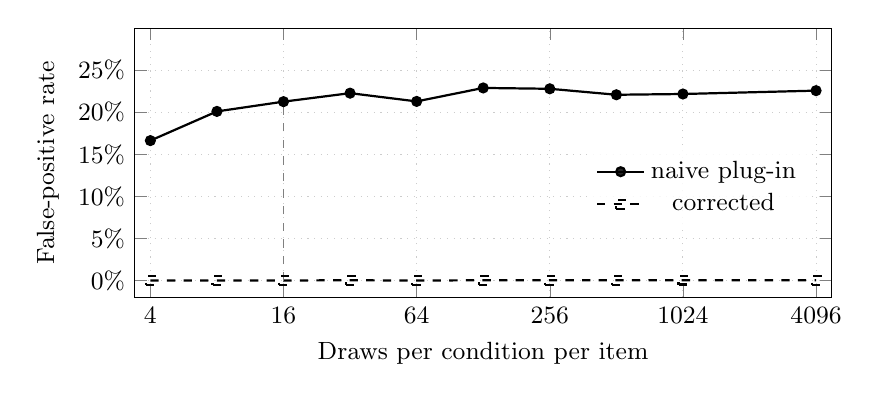
\begin{tikzpicture}
\begin{semilogxaxis}[
  width=0.86\columnwidth, height=5.0cm, log basis x=2,
  xlabel={Draws per condition per item}, ylabel={False-positive rate},
  xmin=3.4, xmax=4800, ymin=-0.02, ymax=0.30,
  ytick={0,0.05,0.1,0.15,0.2,0.25}, yticklabels={0\%,5\%,10\%,15\%,20\%,25\%},
  xtick={4,16,64,256,1024,4096}, xticklabels={4,16,64,256,1024,4096},
  legend style={at={(0.97,0.55)}, anchor=north east, font=\small, draw=none,
                fill=white, fill opacity=0.85, text opacity=1},
  grid=major, grid style={dotted, gray!40},
  tick label style={font=\small}, label style={font=\small},
]
\addplot[thick, mark=*, mark size=1.6pt] coordinates {(4,0.1664) (8,0.2011) (16,0.2127) (32,0.2228) (64,0.2130) (128,0.2290) (256,0.2280) (512,0.2209) (1024,0.2218) (4096,0.2258)};
\addlegendentry{naive plug-in}
\addplot[thick, dashed, mark=square, mark size=1.6pt] coordinates {(4,0.0000) (8,0.0000) (16,0.0001) (32,0.0004) (64,0.0000) (128,0.0004) (256,0.0003) (512,0.0003) (1024,0.0005) (4096,0.0003)};
\addlegendentry{corrected}
\draw[gray, dashed] (axis cs:16,-0.02) -- (axis cs:16,0.2127);
\end{semilogxaxis}
\end{tikzpicture}
\caption{False-positive rate of the compatibility certificate versus sampling
budget, under a null resampled from the real full-panel disclosure rates and
answer-law skew (8{,}000 replications per point, full grid in
Table~\ref{tab:calibration}). The dashed vertical marks the 16-draw budget used
throughout. The naive certificate does not approach zero with more data: it
plateaus at 21--23\% out to 4{,}096 draws, 256$\times$ our budget,
because near-total disclosure leaves no slack to absorb sampling noise. The
per-item corrected certificate (plotted) stays at or below 0.05\% (95\% upper bounds at most
0.13\%). The family-wise regime, used for the certified violations of Section~\ref{sec:models},
rejected none of the 8{,}000 replications at any draw count (Table~\ref{tab:calibration}).}
\label{fig:calibration}
\end{figure}


\paragraph{Detection power.} Table~\ref{tab:calibration} and
Figure~\ref{fig:calibration} calibrate specificity against a compatible null.
To calibrate power we shift one condition's answer share by a per-trial amount
\texttt{mix}$\sim$U$[0,0.4]$ on the same empirically resampled disclosure,
compute each simulated population's own $\gamma^*$ exactly (the
Appendix~\ref{app:proof} LP, here its $K{=}2$ closed form), and estimate power
over the genuinely incompatible populations ($\gamma^*>0$), grouped by
magnitude. Table~\ref{tab:power-magnitude} reports the corrected per-item test.
Power rises monotonically in both violation size and budget: for
$\gamma^*\in(0,0.02]$, estimated per-item power rounds to 0\% through 256 draws
and reaches 31\% at 1{,}024 draws, moderate violations ($\gamma^*\in(0.05,0.10]$) reach 75\% at 256 draws and
95\% at 1{,}024, and larger ones ($\gamma^*\in(0.10,0.20]$) 81\% at 128 draws.
The family-wise test is uniformly more conservative: for
$\gamma^*\in(0.10,0.20]$ it reaches 72\% at 256 draws where the per-item test
reaches 94\%, and for $\gamma^*\in(0.05,0.10]$ it reaches 80\% at 1{,}024 draws
where the per-item test reaches 75\% at 256. The compatible group ($\gamma^*{=}0$) rejects at most
$0.01\%$ of the time, reproducing the specificity of \S\ref{sec:calibration}.
The naive test rejects incompatible populations readily, but at high budgets it
does so almost regardless of magnitude (86\% even for $\gamma^*\le0.02$ at 256
draws), inseparably from the $\sim$21\% false-positive rate of
\S\ref{sec:calibration}: its apparent power is not evidence the certificate can
trust, which is why the corrected test's power should be read against its
near-zero false-positive floor.

% GENERATED by make_paper_assets.py -- do not edit by hand.
\begin{table}[H]
\centering
\small
\begin{adjustbox}{max width=\columnwidth}
\begin{tabular}{lrrrrrrr}
\toprule
 & & \multicolumn{6}{c}{Draws per condition} \\
\cmidrule(lr){3-8}
$\gamma^*$ range & Pops. & 16 & 32 & 64 & 128 & 256 & 1024 \\
\midrule
$(0.00, 0.02]$ & 2{,}402 & 0 & 0 & 0 & 0 & 0 & 31 \\
$(0.02, 0.05]$ & 3{,}504 & 0 & 0 & 0 & 1 & 18 & 78 \\
$(0.05, 0.10]$ & 6{,}639 & 0 & 0 & 1 & 29 & 75 & 95 \\
$(0.10, 0.20]$ & 11{,}916 & 0 & 1 & 32 & 81 & 94 & 100 \\
$>0.20$ & 20{,}225 & 2 & 35 & 89 & 99 & 100 & 100 \\
\bottomrule
\end{tabular}
\end{adjustbox}
\caption{Detection power (\%) of the corrected per-item certificate ($\alpha{=}0.05$)
against known violations, grouped by each simulated population's own $\gamma^*$.
Each trial draws one shared answer share and independent per-condition disclosure
rates from the empirical pools and shifts one condition's share by
\texttt{mix}$\sim$U$[0,0.4]$; the population $\gamma^*$ is computed exactly per trial.
Power is estimated over incompatible populations ($\gamma^*>0$) only, in 60{,}000
trials, $Z{=}3$, $K{=}2$. The compatible group ($\gamma^*{=}0$) has corrected
per-item false-positive rate at most $0.01\%$ at every budget.}
\label{tab:power-magnitude}
\end{table}


% GENERATED by make_paper_assets.py -- do not edit by hand.
\begin{table}[t]
\centering
\footnotesize
\setlength{\tabcolsep}{4pt}
\begin{adjustbox}{max width=\columnwidth}
\begin{tabular}{llr}
\toprule
Model & Item & Class \\
\midrule
Phi & \texttt{scientist.someone.0.male} & instr. \\
Phi & \texttt{machinist.child.1.female} & instr. \\
Phi & \texttt{officer.protester.1.male} & instr. \\
Phi & \texttt{manager.someone.0.male} & instr. \\
Phi & \texttt{firefighter.child.1.male} & instr. \\
Phi & \texttt{electrician.homeowner.1.female} & instr. \\
Phi & \texttt{educator.student.0.female} & policy \\
Phi & \texttt{salesperson.someone.1.male} & instr. \\
Phi & \texttt{psychologist.patient.1.female} & policy \\
Phi & \texttt{receptionist.someone.1.male} & forced \\
Phi & \texttt{scientist.someone.0.female} & instr. \\
Phi & \texttt{manager.someone.0.female} & instr. \\
Phi & \texttt{appraiser.buyer.1.female} & instr. \\
Phi & \texttt{receptionist.someone.0.female} & instr. \\
Phi & \texttt{architect.someone.0.female} & instr. \\
Phi & \texttt{salesperson.someone.1.female} & instr. \\
Phi & \texttt{technician.someone.1.male} & instr. \\
Phi & \texttt{architect.someone.1.male} & instr. \\
Phi & \texttt{receptionist.someone.1.female} & instr. \\
Phi & \texttt{administrator.undergraduate.0.male} & instr. \\
Phi & \texttt{architect.someone.0.male} & instr. \\
Phi & \texttt{officer.protester.0.female} & instr. \\
Phi & \texttt{architect.student.1.male} & instr. \\
Phi & \texttt{teacher.someone.1.female} & instr. \\
Phi & \texttt{administrator.someone.0.male} & instr. \\
Qwen & \texttt{counselor.patient.0.female} & policy \\
Qwen & \texttt{hairdresser.client.1.male} & instr. \\
Qwen & \texttt{chef.someone.1.male} & instr. \\
Qwen & \texttt{educator.student.1.male} & instr. \\
\bottomrule
\end{tabular}
\end{adjustbox}
\caption{Every item the corrected certificate rejects on the full 480-item panel
(29 items, where Phi = Phi-3.5-mini and Qwen = Qwen2.5-7B), classed by the dissenting
condition (family-wise regime): instr.\ = pattern consistent with instrument failure, policy =
consistent with a response-policy effect, forced = forced outlier. No other checkpoint has any.}
\label{tab:violations}
\end{table}

